\documentclass[10pt]{article}
\usepackage[a4paper,margin=18mm,top=16mm,bottom=16mm]{geometry}
\usepackage[scaled=0.92]{helvet}\renewcommand{\familydefault}{\sfdefault}
\usepackage[T1]{fontenc}\usepackage{amsmath,booktabs,array,xcolor,titlesec,enumitem,caption,float}
\usepackage{graphicx}\graphicspath{{./}{../figures/}}
\usepackage{pgfplots}\usepgfplotslibrary{groupplots}\pgfplotsset{compat=1.15}
\titleformat{\section}{\normalsize\bfseries}{\thesection}{0.6em}{}\titlespacing*{\section}{0pt}{10pt}{3pt}
\setlength{\parindent}{0pt}\setlength{\parskip}{3pt}\captionsetup{font=small,labelfont=bf,skip=4pt}
\setlist{nosep,leftmargin=1.2em,itemsep=3pt}\pagestyle{empty}
\newcommand{\todo}[1]{\textcolor{red}{[#1]}}
\definecolor{ink}{HTML}{0B0B0B}\definecolor{muted}{HTML}{52514E}\definecolor{gridc}{HTML}{DDDCD6}\definecolor{bandc}{HTML}{EEEDE8}
\definecolor{otherc}{HTML}{A3A29B}\definecolor{cA}{HTML}{2A78D6}\definecolor{cB}{HTML}{EB6834}\definecolor{cC}{HTML}{1BAF7A}
\pgfplotsset{
  ds/.style={line width=0.7pt, mark=*, mark size=1.25pt},
  other/.style={otherc, line width=0.5pt, mark=*, mark size=1.1pt, mark options={fill=otherc, draw=white, line width=0.2pt}},
  hi/.style={line width=1.1pt, mark=*, mark size=1.9pt, mark options={draw=white, line width=0.4pt}},
  sA/.style={cA, mark options={fill=cA, draw=white, line width=0.4pt}},
  sB/.style={cB, mark options={fill=cB, draw=white, line width=0.4pt}},
  sC/.style={cC, mark options={fill=cC, draw=white, line width=0.4pt}}}
\begin{document}
{\large\bfseries BudgetMesh: what we compare against, and why}\\[1pt]
{\small All numbers are measured runs. 13 Nov 2026.}

\section{The main comparison}
\begin{figure}[H]\centering
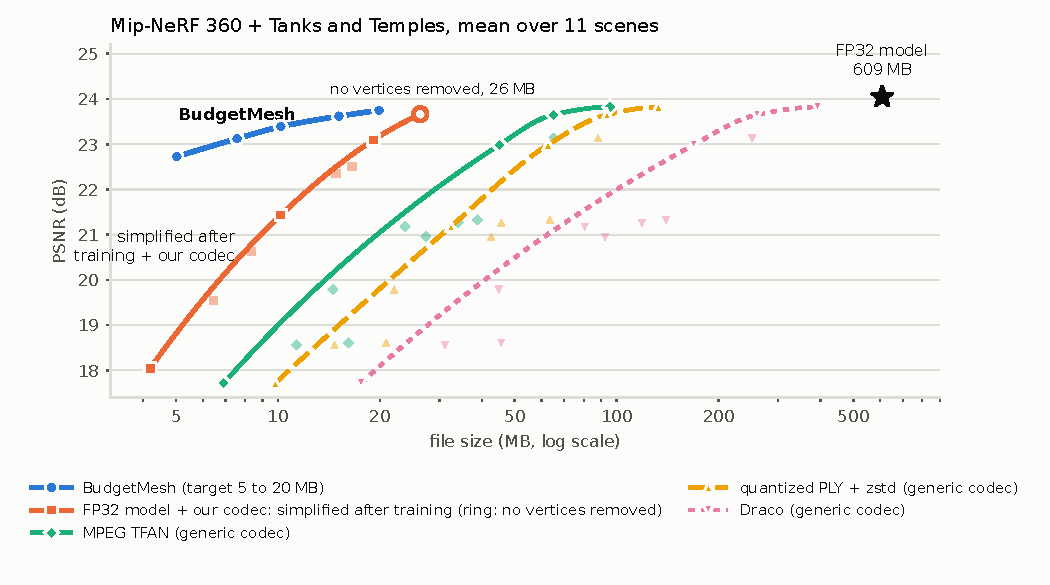
\includegraphics[width=0.86\textwidth]{fig_rd_system_v1.pdf}
\caption{Quality (PSNR) against file size. Mean of 11 captured scenes (Mip-NeRF 360, Tanks and Temples). Each curve keeps the best points of its method.}\label{fig:rd}
\end{figure}

\textbf{What each curve is.}
\begin{itemize}
\item \textbf{FP32 model (star).} MeshSplatting as released, default settings, saved with no compression. 609\,MB.
\item \textbf{Draco (pink).} Google's mesh compressor, used as it is. We give it the MeshSplatting mesh at full size and at three smaller sizes (vertices removed after training, then fine-tuned). Colours are stored with 8, 6 or 4 bits.
\item \textbf{MPEG TFAN (green).} The MPEG mesh compressor, used as it is. Same meshes as Draco.
\item \textbf{Quantized PLY + zstd (yellow).} Round the numbers, write them to a PLY file, compress the file with zstd, a general-purpose compressor. Same meshes as Draco.
\item \textbf{FP32 model + our codec (orange).} The same kind of mesh again: the MeshSplatting mesh, at full size (the ring) and with vertices removed after training. Only the compressor is different: ours.
\item \textbf{BudgetMesh (blue).} Our full system. The mesh is brought to the target size while it is still training, then compressed with our codec.
\end{itemize}

\textbf{What the figure shows.}
\begin{enumerate}
\item \textbf{As a codec, ours compresses better.} Orange against green, yellow and pink: the meshes are the same, only the compressor changes. For the full-size mesh at about 23.65\,dB, our file is 26\,MB, TFAN's is 65\,MB, zstd's is 94\,MB and Draco's is 260\,MB. Over the whole curve we are 2.4 to 2.5 times smaller than TFAN, the best of the three.
\item \textbf{The size has to be controlled during training.} Blue against orange: the compressor is the same, the only difference is when the mesh is brought to size. At 5, 10 and 20\,MB, sizing during training is 4.0, 2.0 and 0.6\,dB better than removing vertices after training.
\item \textbf{Both together.} For the same PSNR, TFAN needs 4.1 to 8.2 times more bytes than BudgetMesh. This number contains both gains, the codec and the sizing during training.
\end{enumerate}

\section{Why we do not build more baselines of our own}
\begin{itemize}
\item Any baseline needs a trained scene. A trained scene comes from the original MeshSplatting. The only handle on size there is the vertex cap.
\item In the released code the cap is one fixed number, 4 million vertices, the same for every scene. It is a ceiling, not a way to choose a file size.
\item We are the ones who started tuning it, because it is the most direct handle on the number of vertices.
\item It does not behave like a size setting (Figure~\ref{fig:cap}). Without trying several caps on a scene, nobody can know which cap gives which size, and a cap found on one scene does not carry over to another.
\item Taking the cap from other scenes of the same dataset (a prior) is not a fair comparison either. Our method is given only the scene and the target size.
\item So the vertex cap is not a baseline. It is one row in the ablation and it answers one question: \emph{how much better is the controller than tuning the cap by hand?}
\end{itemize}

\begin{figure}[H]\centering
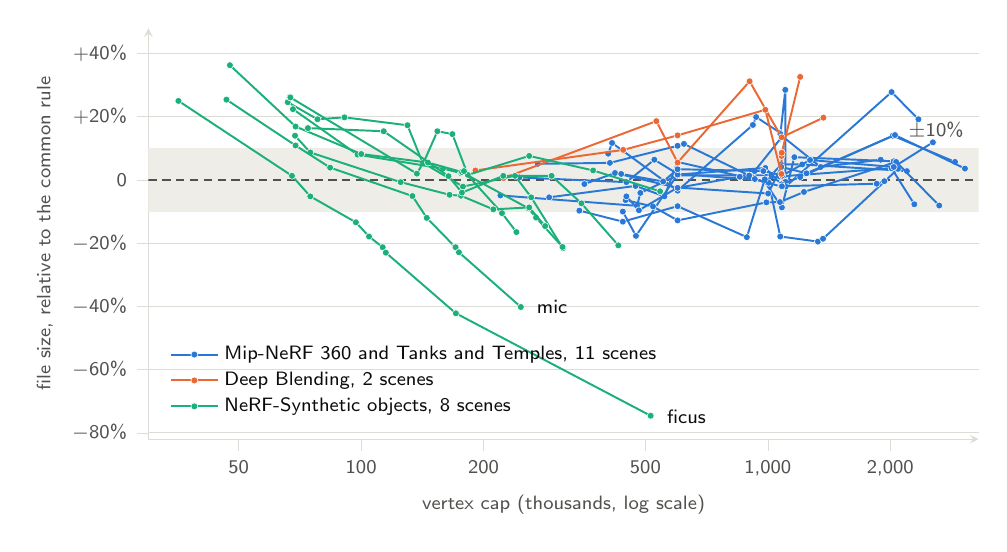
\begin{tikzpicture}
\begin{axis}[width=\textwidth, height=68mm, xmode=log, log ticks with fixed point,
  xmin=30, xmax=3300, ymin=-82, ymax=48, xtick={50,100,200,500,1000,2000}, ytick={-80,-60,-40,-20,0,20,40},
  xticklabels={50,100,200,500,{1,000},{2,000}}, yticklabels={$-$80\%,$-$60\%,$-$40\%,$-$20\%,0,+20\%,+40\%}, minor tick style={draw=none},
  axis lines=left, axis line style={gridc}, tick style={gridc}, tick align=outside, tick label style={font=\scriptsize, text=muted},
  label style={font=\scriptsize, text=muted}, ymajorgrids, grid style={gridc, line width=0.3pt}, clip=true, clip marker paths=true,
  xlabel={vertex cap (thousands, log scale)}, ylabel={file size, relative to the common rule},
  legend style={font=\scriptsize, text=ink, draw=none, fill=none, at={(0.015,0.03)}, anchor=south west, row sep=-1pt}, legend cell align=left]
\path[fill=bandc] (axis cs:30,-10) rectangle (axis cs:3300,10);
\draw[muted, line width=0.5pt, dash pattern=on 3pt off 2pt] (axis cs:30,0) -- (axis cs:3300,0);
\addlegendimage{ds, cA, mark options={fill=cA, draw=white, line width=0.2pt}}\addlegendentry{Mip-NeRF 360 and Tanks and Temples, 11 scenes}
\addlegendimage{ds, cB, mark options={fill=cB, draw=white, line width=0.2pt}}\addlegendentry{Deep Blending, 2 scenes}
\addlegendimage{ds, cC, mark options={fill=cC, draw=white, line width=0.2pt}}\addlegendentry{NeRF-Synthetic objects, 8 scenes}
\addplot[ds, cA, mark options={fill=cA, draw=white, line width=0.2pt}, forget plot] coordinates {(220.000,-4.9) (477.000,-8.2) (486.000,-4.1) (600.000,1.4) (1020.000,1.5) (1078.000,4.9) (1215.000,4.9) (2198.000,2.8)}; % room
\addplot[ds, cA, mark options={fill=cA, draw=white, line width=0.2pt}, forget plot] coordinates {(272.000,5.1) (409.000,5.4) (600.000,10.8) (622.000,11.4) (900.000,1.4) (928.000,2.8) (1086.000,13.8) (1349.000,4.1) (1895.000,6.4)}; % kitchen
\addplot[ds, cA, mark options={fill=cA, draw=white, line width=0.2pt}, forget plot] coordinates {(245.000,0.8) (449.000,-0.7) (526.000,6.4) (600.000,1.9) (978.000,-0.2) (1083.000,-8.7) (1162.000,7.2) (2040.000,5.9)}; % counter
\addplot[ds, cA, mark options={fill=cA, draw=white, line width=0.2pt}, forget plot] coordinates {(290.000,-5.5) (473.000,-1.9) (557.000,-5.2) (600.000,5.7) (1005.000,-0.9) (1073.000,-17.9) (1328.000,-19.5) (1367.000,-18.6) (2090.000,3.5)}; % bonsai
\addplot[ds, cA, mark options={fill=cA, draw=white, line width=0.2pt}, forget plot] coordinates {(405.000,8.3) (414.000,11.7) (600.000,-3.4) (919.000,17.4) (936.000,19.9) (1073.000,14.9) (1074.000,14.5) (1104.000,28.5) (1105.000,-0.6) (1106.000,-2.1) (2015.000,27.8) (2346.000,19.2)}; % garden
\addplot[ds, cA, mark options={fill=cA, draw=white, line width=0.2pt}, forget plot] coordinates {(440.000,-10.0) (474.000,-17.7) (600.000,1.7) (986.000,3.8) (1080.000,-1.4) (1201.000,0.9) (2029.000,14.0) (2886.000,5.7)}; % bicycle
\addplot[ds, cA, mark options={fill=cA, draw=white, line width=0.2pt}, forget plot] coordinates {(344.000,-9.7) (440.000,-13.2) (600.000,-8.3) (888.000,-18.1) (983.000,0.2) (1069.000,1.1) (2015.000,3.7) (2292.000,-7.7)}; % stump
\addplot[ds, cA, mark options={fill=cA, draw=white, line width=0.2pt}, forget plot] coordinates {(447.000,-6.4) (522.000,-8.4) (600.000,-12.8) (992.000,-7.1) (1071.000,-7.0) (1227.000,-3.8) (2068.000,5.7) (2639.000,-8.1)}; % flowers
\addplot[ds, cA, mark options={fill=cA, draw=white, line width=0.2pt}, forget plot] coordinates {(449.000,-5.2) (482.000,-9.6) (600.000,-2.4) (1002.000,-4.3) (1079.000,4.1) (1245.000,2.1) (2054.000,14.2) (3053.000,3.6)}; % treehill
\addplot[ds, cA, mark options={fill=cA, draw=white, line width=0.2pt}, forget plot] coordinates {(354.000,-1.3) (421.000,2.2) (600.000,-2.5) (853.000,1.0) (929.000,0.3) (1078.000,-2.1) (1083.000,-2.0) (1853.000,-1.2) (1934.000,-0.4)}; % truck
\addplot[ds, cA, mark options={fill=cA, draw=white, line width=0.2pt}, forget plot] coordinates {(436.000,1.9) (553.000,-0.5) (600.000,3.4) (975.000,2.8) (1085.000,1.4) (1270.000,6.3) (2040.000,4.1) (2546.000,11.9)}; % train
\addplot[ds, cB, mark options={fill=cB, draw=white, line width=0.2pt}, forget plot] coordinates {(224.000,0.6) (532.000,18.6) (600.000,5.5) (902.000,31.2) (1081.000,13.5) (1370.000,19.7)}; % drjohnson
\addplot[ds, cB, mark options={fill=cB, draw=white, line width=0.2pt}, forget plot] coordinates {(191.000,3.0) (441.000,9.5) (600.000,14.1) (986.000,22.2) (1080.000,1.9) (1081.000,7.6) (1082.000,8.6) (1201.000,32.6)}; % playroom
\addplot[ds, cC, mark options={fill=cC, draw=white, line width=0.2pt}, forget plot] coordinates {(66.000,24.6) (78.124,19.2) (91.000,19.8) (130.000,17.3) (142.000,5.1) (154.000,15.4) (167.656,14.5) (183.000,1.6) (259.000,7.6) (372.025,3.0) (543.482,-3.6)}; % lego
\addplot[ds, cC, mark options={fill=cC, draw=white, line width=0.2pt}, forget plot] coordinates {(66.755,26.2) (67.000,26.1) (137.117,2.0) (142.000,5.4) (178.000,-2.1) (238.956,1.3) (262.000,-5.5) (313.435,-21.6)}; % chair
\addplot[ds, cC, mark options={fill=cC, draw=white, line width=0.2pt}, forget plot] coordinates {(68.000,22.4) (97.992,8.0) (159.000,3.6) (175.593,2.2) (176.000,2.6) (258.000,-9.0) (269.192,-11.9) (312.716,-21.2)}; % drums
\addplot[ds, cC, mark options={fill=cC, draw=white, line width=0.2pt}, forget plot] coordinates {(35.557,25.0) (67.614,1.3) (75.000,-5.2) (97.082,-13.4) (104.589,-17.9) (113.000,-21.3) (115.000,-23.0) (171.000,-42.2) (515.000,-74.6)}; % ficus
\addplot[ds, cC, mark options={fill=cC, draw=white, line width=0.2pt}, forget plot] coordinates {(47.578,36.3) (69.000,16.9) (100.090,8.2) (146.000,5.5) (177.000,2.5) (179.024,2.8) (222.000,-10.5) (240.925,-16.5)}; % hotdog
\addplot[ds, cC, mark options={fill=cC, draw=white, line width=0.2pt}, forget plot] coordinates {(68.793,14.0) (75.000,8.7) (125.118,-0.7) (165.000,-4.7) (176.000,-5.0) (211.349,-9.3) (259.000,-8.7) (283.400,-14.6)}; % materials
\addplot[ds, cC, mark options={fill=cC, draw=white, line width=0.2pt}, forget plot] coordinates {(46.659,25.4) (69.000,10.9) (83.900,3.9) (133.718,-5.1) (145.000,-12.0) (170.000,-21.1) (170.724,-21.3) (174.000,-22.9) (247.000,-40.2)}; % mic
\addplot[ds, cC, mark options={fill=cC, draw=white, line width=0.2pt}, forget plot] coordinates {(74.000,16.4) (113.638,15.4) (164.000,1.2) (177.000,-4.0) (223.635,1.3) (294.000,1.3) (348.124,-7.4) (428.970,-20.7)}; % ship
\node[font=\scriptsize, text=muted, anchor=south east] at (axis cs:3200,10) {$\pm$10\%};
\node[font=\scriptsize, text=ink, anchor=west] at (axis cs:535,-75) {ficus};
\node[font=\scriptsize, text=ink, anchor=west] at (axis cs:256,-40) {mic};
\end{axis}
\end{tikzpicture}
\caption{Every cap run of all 21 scenes on one pair of axes. The common rule is the best single curve that turns a cap into a file size for all scenes together (file in MB = 0.0588 $\times$ cap in thousands to the power 0.738, fitted on these same runs). If the cap decided the file size, every point would sit on the dashed line. 114 of the 178 runs are within $\pm$10\% of it (light band); the others are between $-$75\% and +36\%.}\label{fig:cap}
\end{figure}

\begin{itemize}
\item \textbf{No single rule turns a cap into a size.} Even the best common rule, fitted on these very runs, misses by more than 10\% in 64 of 178 runs. With one rule per dataset it is still 27 of 109 runs on captured scenes and 29 of 69 on objects.
\item \textbf{Same cap, different scenes, different sizes.} With a cap of exactly 600,000 the 13 captured scenes give files from 5.8 to 7.5\,MB. With a cap of about 1.08 million they give 8.3 to 11.6\,MB. With a cap of about 176 thousand the 8 objects give files from 1.5 to 2.8\,MB.
\item \textbf{Same scene, almost the same cap, different sizes.} Garden: a cap of 1,104,000 gives 13.3\,MB, a cap of 1,105,000 gives 10.3\,MB.
\item \textbf{A larger cap can give a smaller file.} Bonsai: 1,005,000 gives 9.6\,MB, 1,073,000 gives 8.3\,MB.
\item \textbf{Raising the cap can do nothing.} Mic stays at about 2.05\,MB from a cap of 134 thousand up to 247 thousand. Ficus stays at 1.5\,MB from 97 thousand up to 515 thousand.
\item \textbf{Over all cap runs.} Take two runs of the same scene whose caps are less than 1\% apart: 11 such pairs, and in 4 of them the larger cap gave the smaller file. Less than 5\% apart: 29 pairs, 12 with the larger cap giving the smaller file, 8 with the file changing by more than 10\%.
\end{itemize}

\section{The ablation: controller against tuning the cap by hand}
\textbf{How we count.}
\begin{itemize}
\item Both sides get the same input: the scene and the target size. Nothing from other scenes.
\item Without a prior, the cap user must first run the released default (cap 4 million) once to see how large the scene is. We call this run 0, and its time is counted.
\item Then come the capped trainings, until the file is within $\pm$10\% of the target, at most three.
\item Time for the cap = run 0 + all capped trainings. We report the slowest scene (worst case). Encoding time is reported separately for both sides.
\end{itemize}

\textbf{What is measured so far.} 21 scenes, one target each: 10\,MB for the 13 captured scenes, 2.5\,MB for the 8 objects. In these runs the cap was still taken from other scenes of the same dataset, so the cap column had help that the rules above do not allow.

\begin{table}[H]\centering\small
\begin{tabular}{@{}lcc@{}}
\toprule
 & Vertex cap, tuned by hand & Controller (ours) \\
\midrule
Within $\pm$10\% after 1 training & 15 / 21 & 20 / 21 \\
Within $\pm$10\% after 3 trainings & 18 / 21 & 20 / 21 (never retrains) \\
Within $\pm$2\% after 1 training & 3 / 21 & 16 / 21 \\
Never within $\pm$10\% & drjohnson, mic, ficus & ficus \\
PSNR at the same file size & reference & +0.33\,dB (better in 34 of 36) \\
Slowest scene that reached $\pm$10\% & 81 min, 2 trainings, run 0 not yet added & 71 min, 1 training \\
\bottomrule
\end{tabular}
\end{table}
\vspace{-4pt}
Still to add: \todo{time of run 0 for each scene, added to the cap column} and \todo{encoding time for both columns}.
\end{document}
